\documentclass[a4paper,12pt]{book}
\usepackage[utf8]{inputenc}
\usepackage{graphicx}
\usepackage{pdfpages}

\renewcommand\thesection{\arabic{section}}


\begin{document}

\author{E. F. Haghish}
\title{MarkDoc (\texttt{4.0}) Stata Help Files}
\date{October 2018}

\frontmatter
\maketitle
\tableofcontents

\mainmatter

%\includegraphics[width=107mm, scale=0.5]{images/qplot}
\section{\texttt{markdoc}} \label{markdoc}
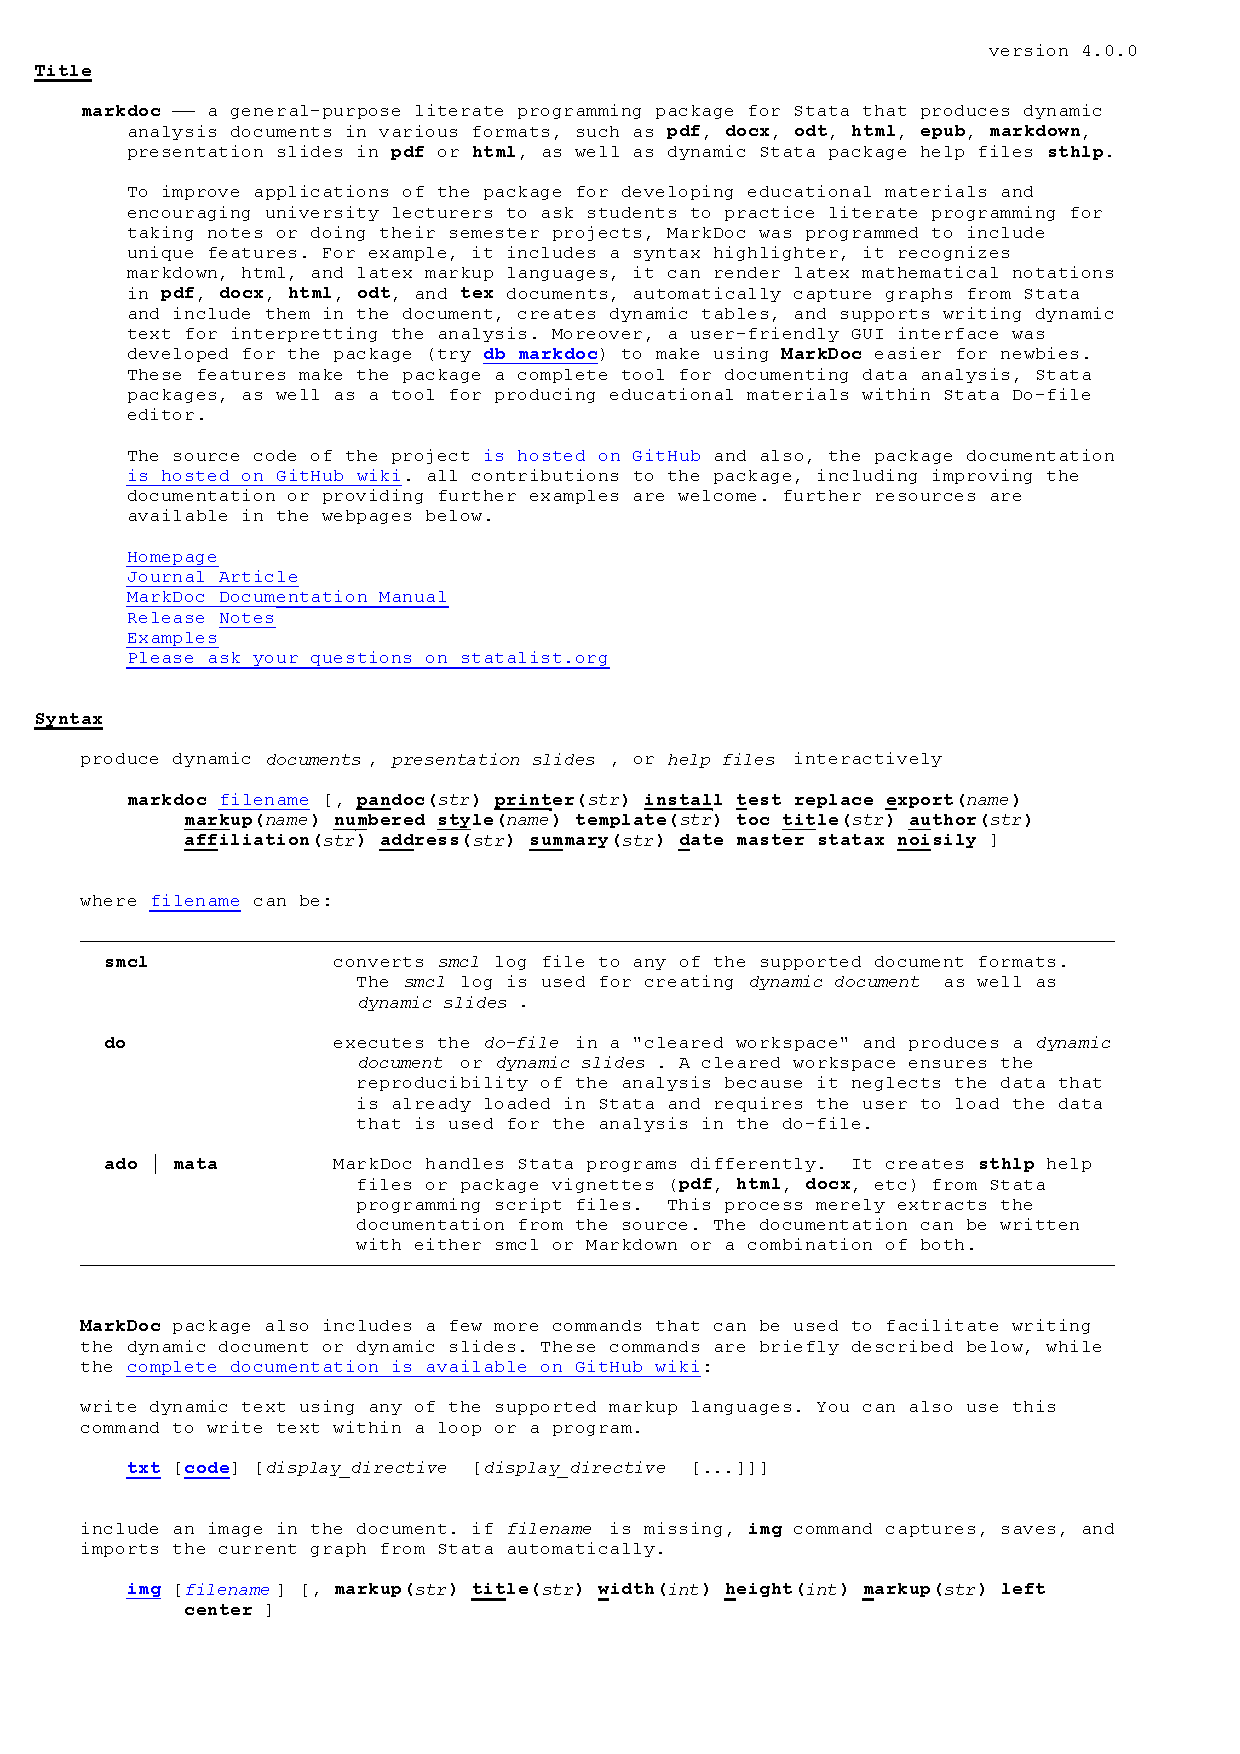
\includepdf[pages={1-}]{helpfiles/markdoc}

\section{Additional programs} \label{additional programs}
\subsection{\texttt{txt}} \label{txt}
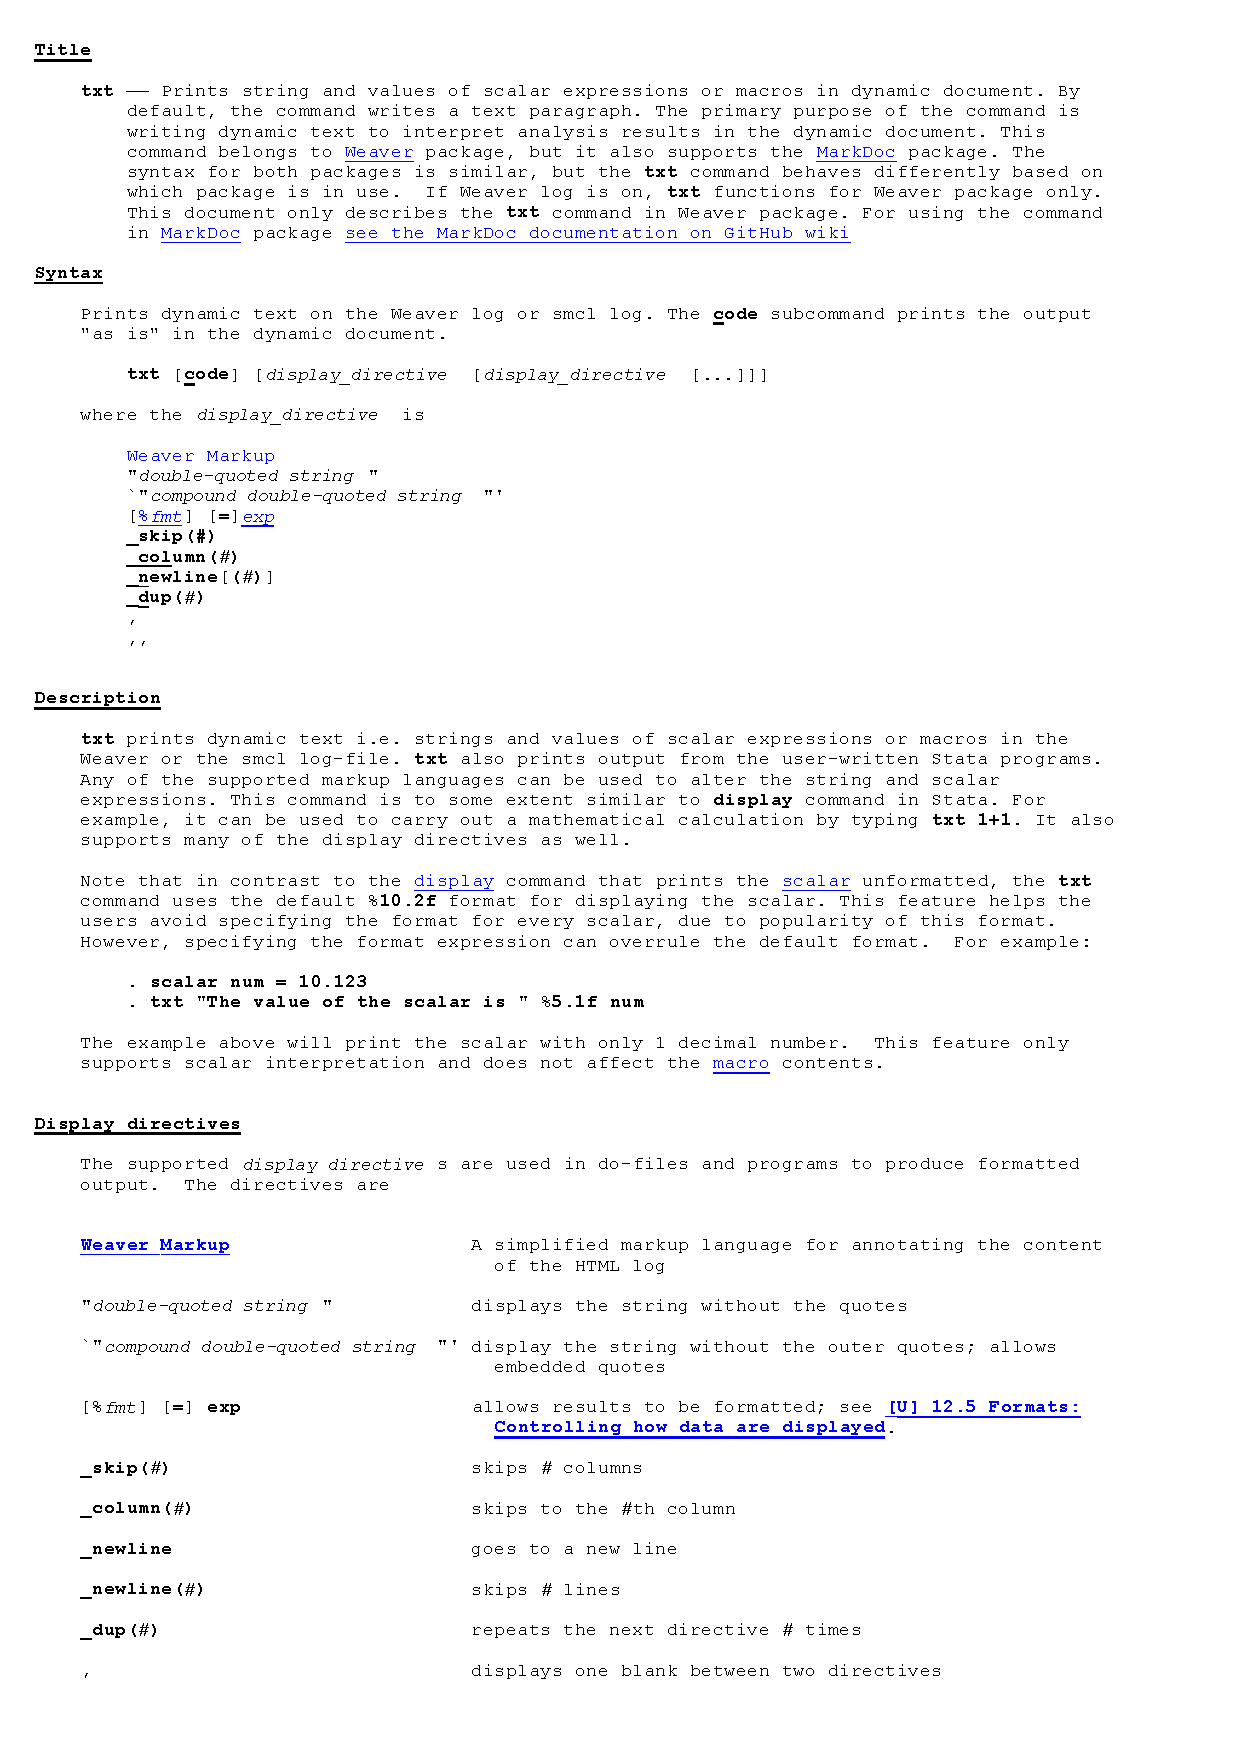
\includepdf[pages={1-}]{helpfiles/txt}
\subsection{\texttt{img}} \label{img}
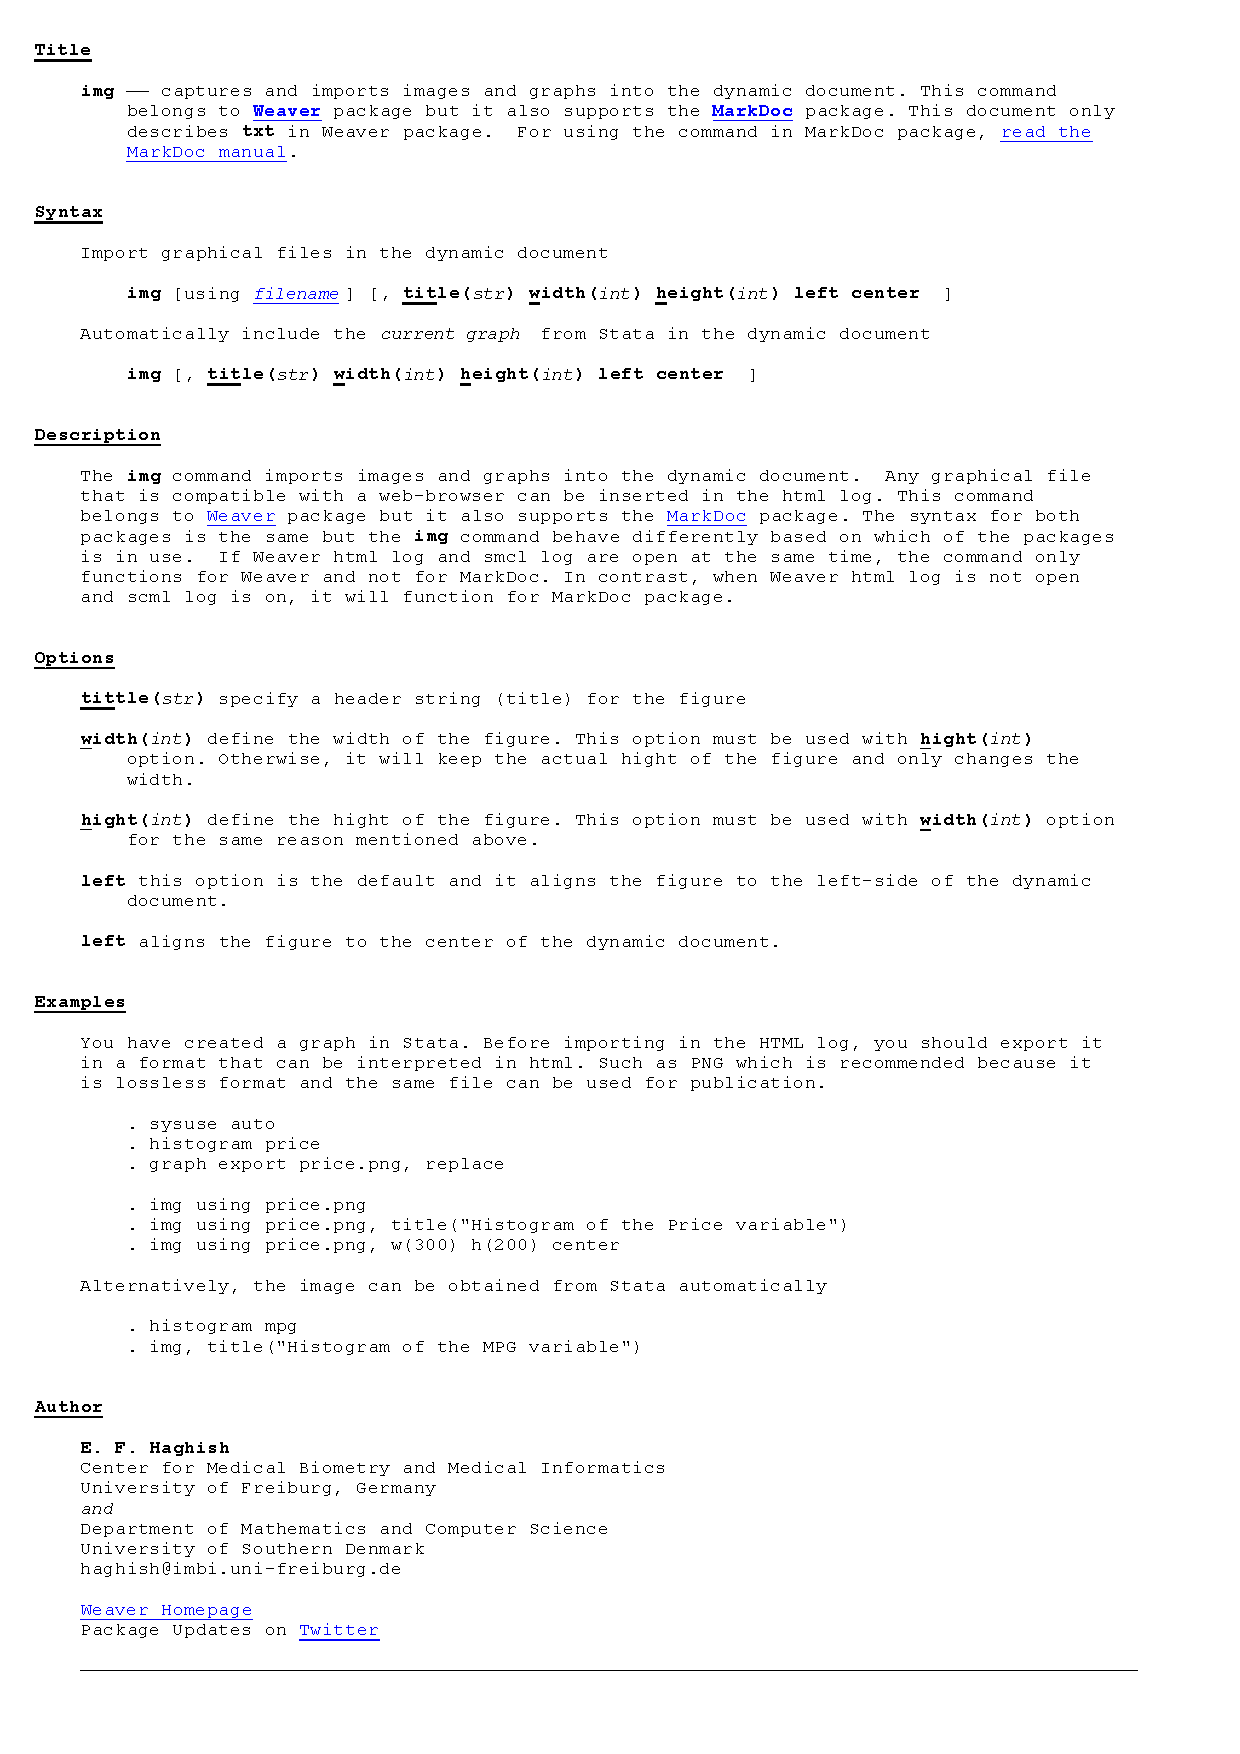
\includepdf[pages={1-}]{helpfiles/img}
\subsection{\texttt{tbl}} \label{tbl}
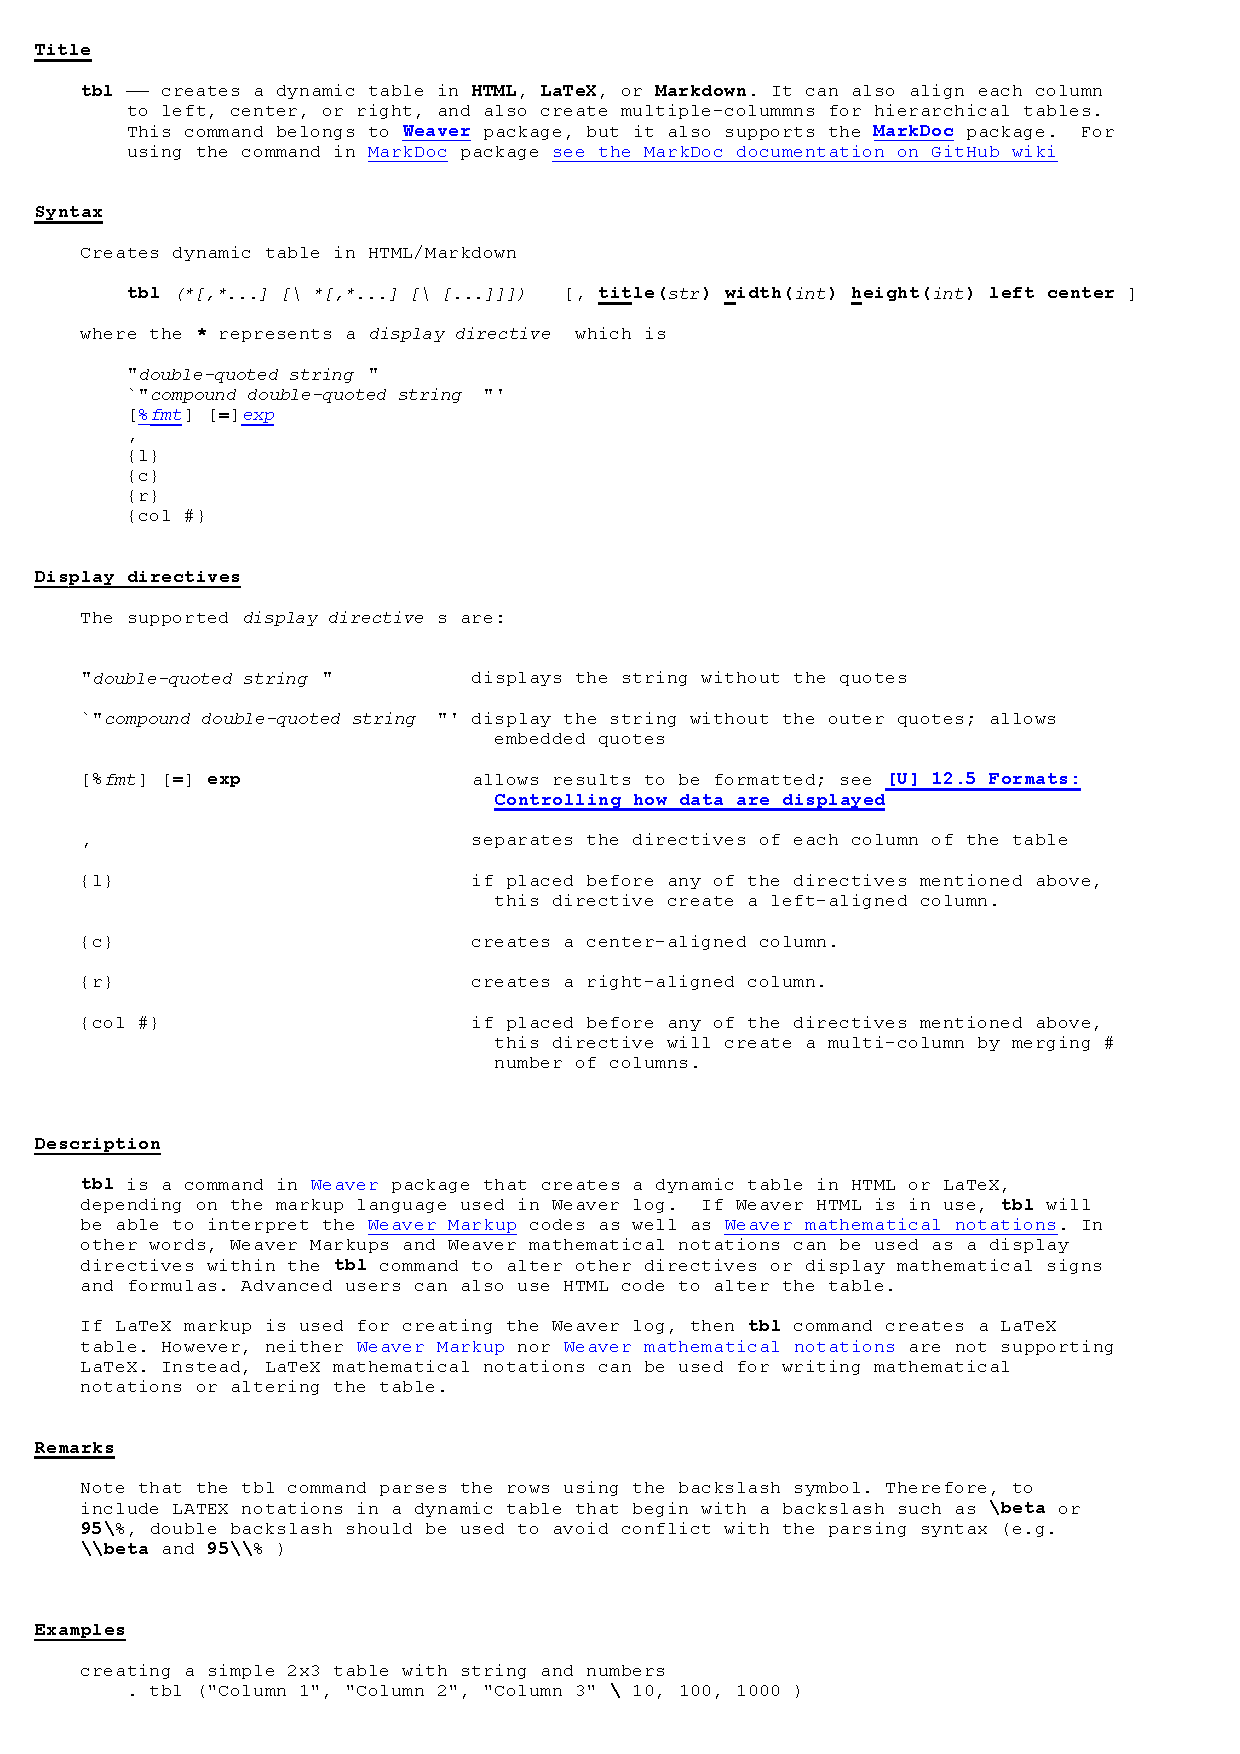
\includepdf[pages={1-}]{helpfiles/tbl}
\section{Calling third-party software within Stata} \label{Calling third-party software within Stata}
\subsection{\texttt{pandoc}} \label{pandoc}
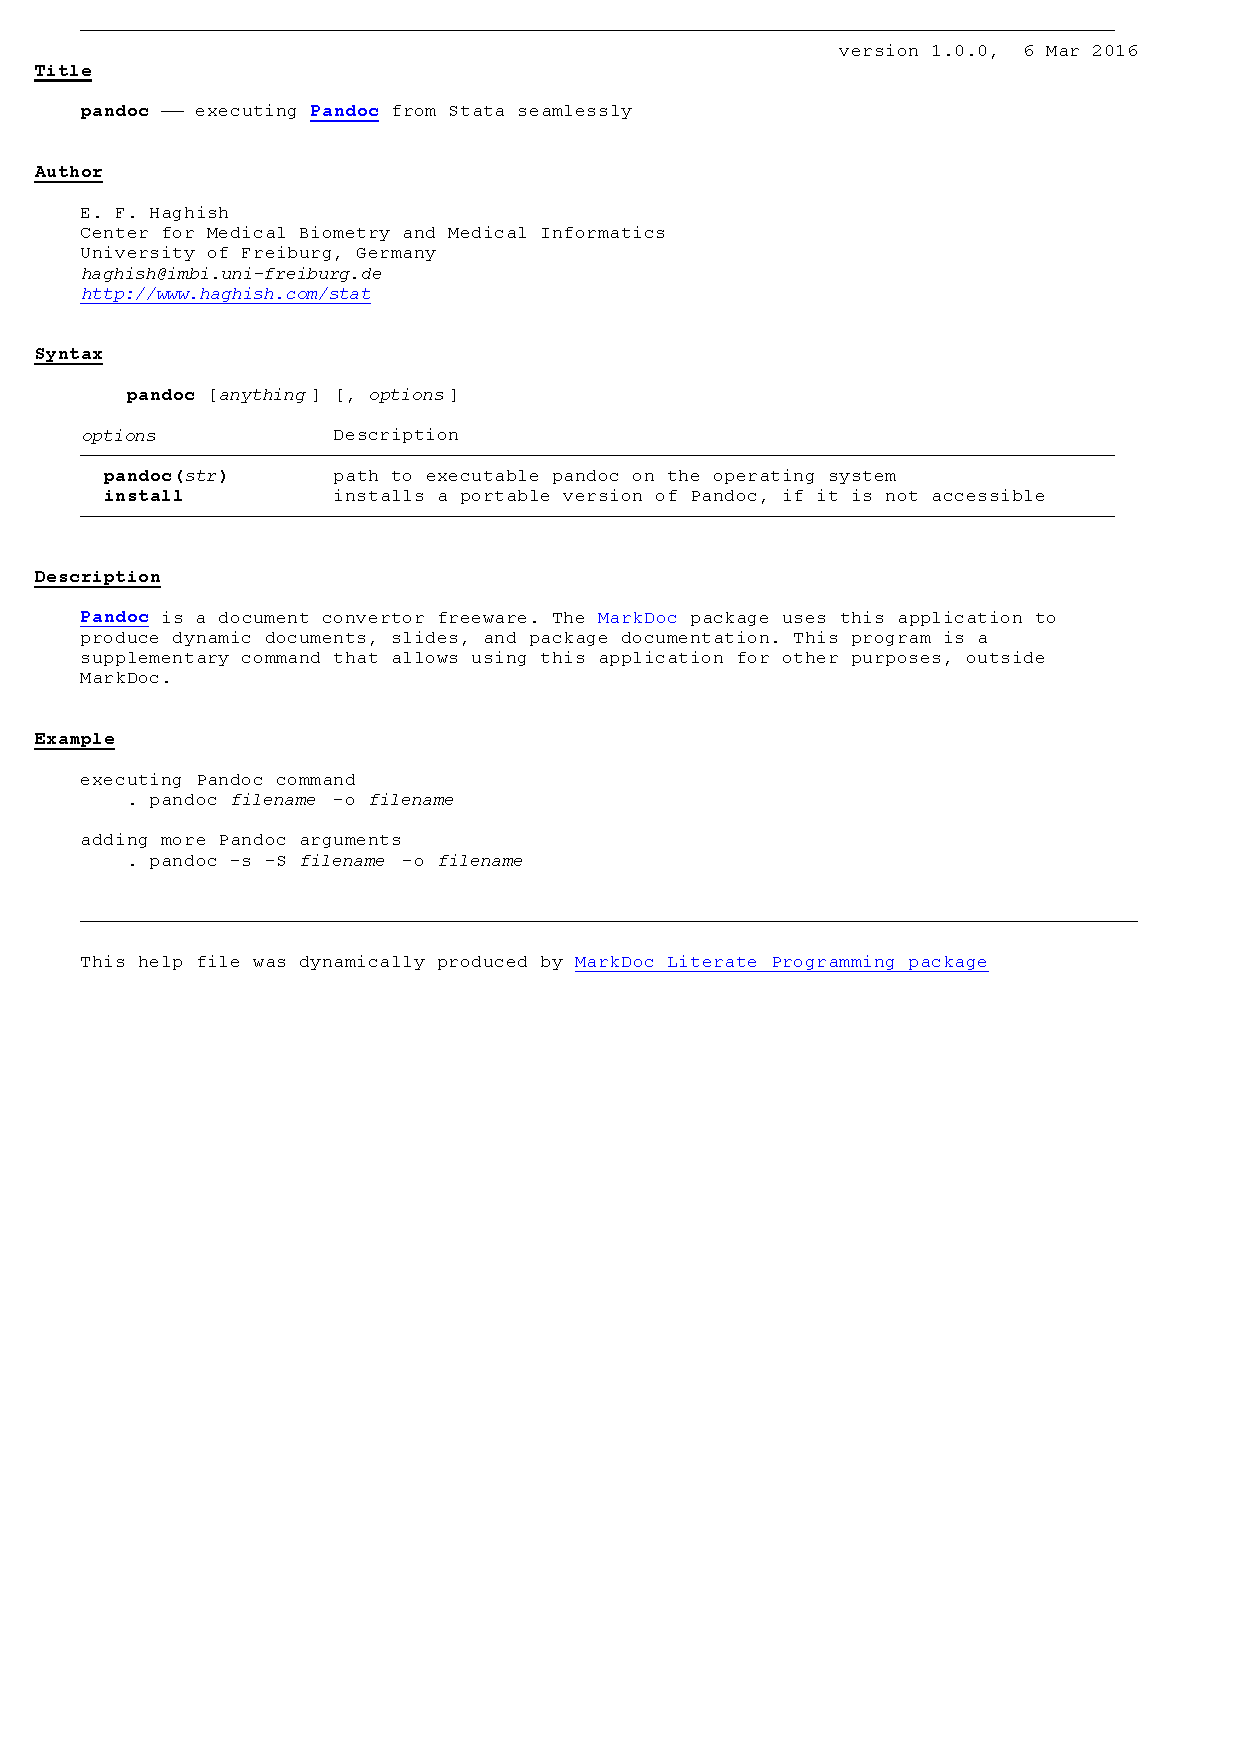
\includepdf[pages={1-}]{helpfiles/pandoc}
\subsection{\texttt{wkhtmltopdf}} \label{wkhtmltopdf}
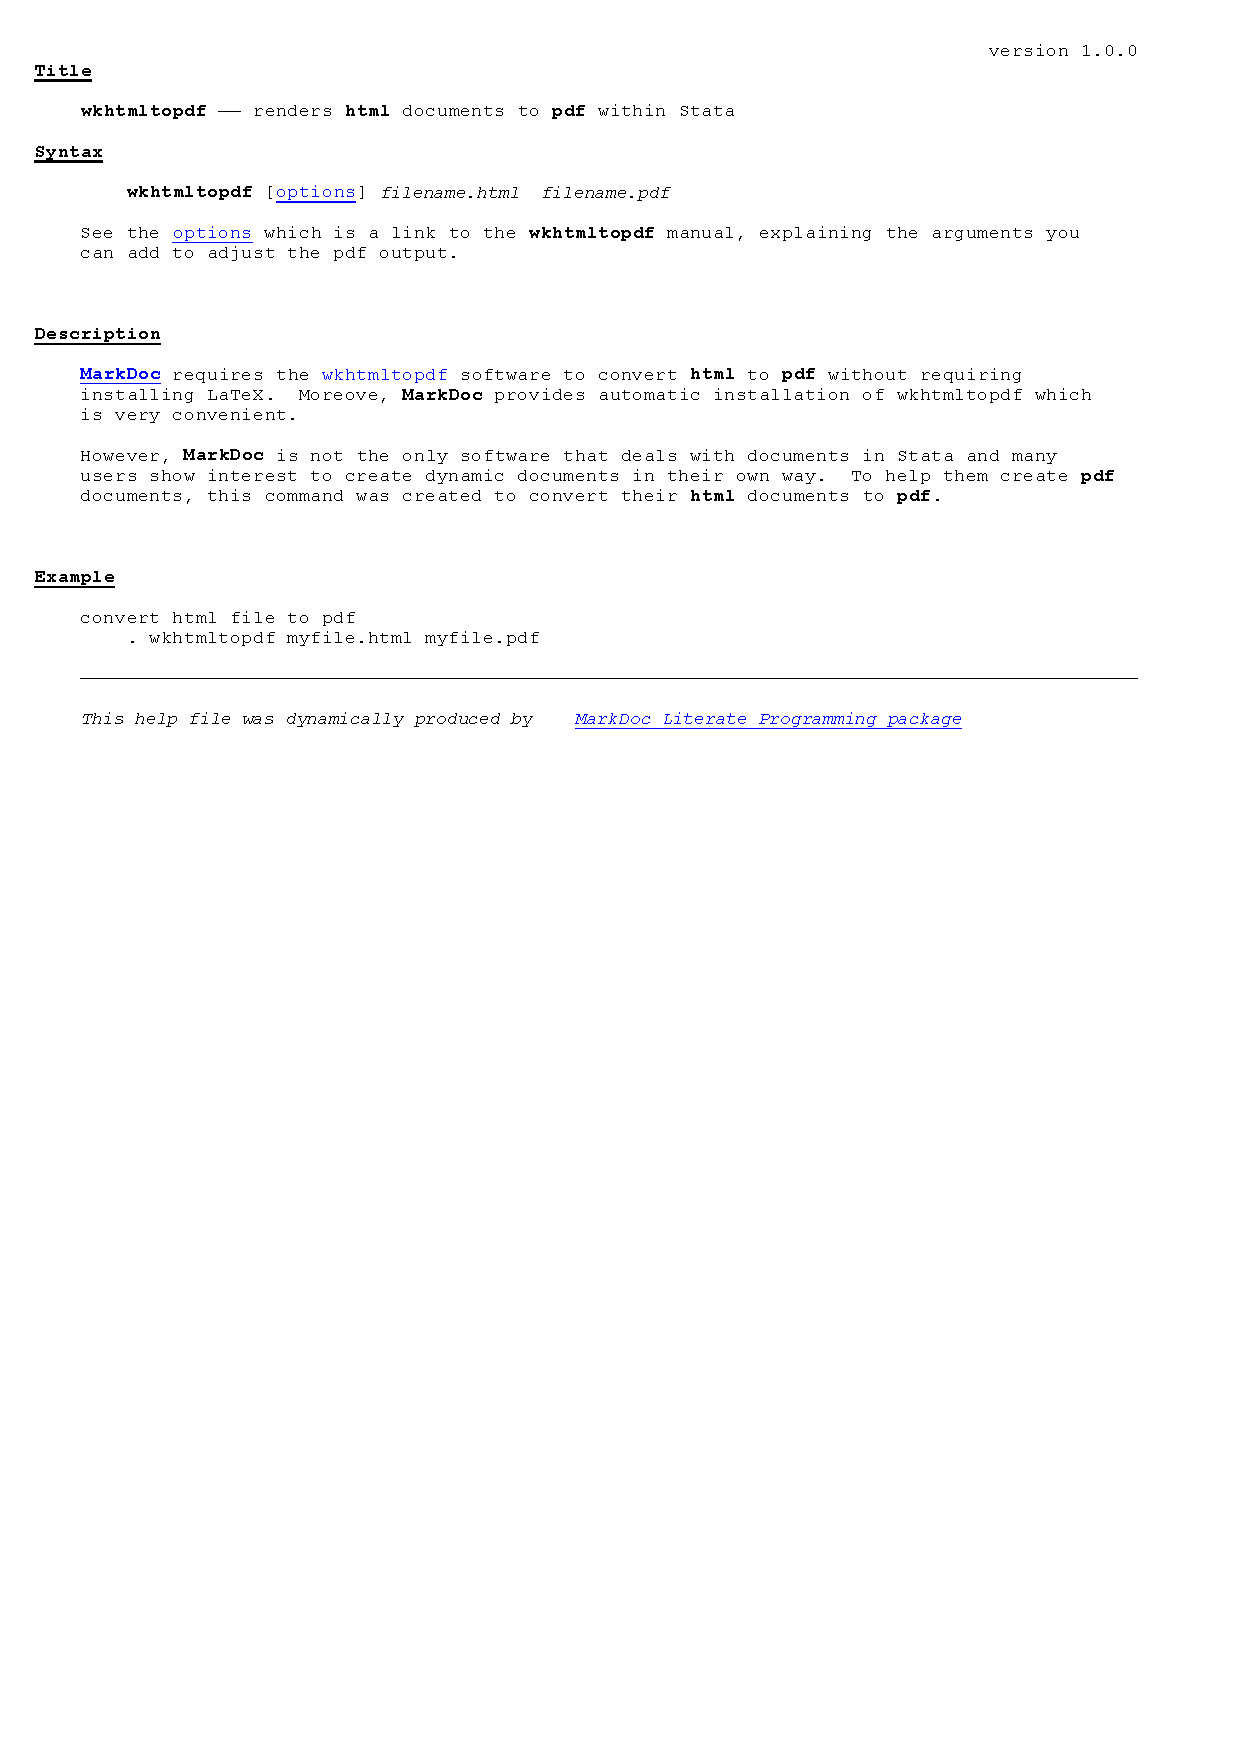
\includepdf[pages={1-}]{helpfiles/wkhtmltopdf}




%\include{./TeX_files/chapter01}
%\include{./TeX_files/chapter02}

\backmatter
% bibliography, glossary and index would go here.

\end{document}